
\section{Единственность классического решения задачи Коши для уравнения
теплопроводности в классе $\mathbf{M_2(T)}$.}
%Никитушка отмочил красоту

{\bf Единственность решения задачи Коши}\\
Вообще говоря, решение единственным будет не всегда. Но если
 ограничиться некоторым классом функций, то в нем решение может
  оказаться единственным. Введем такой класс.\\
  
  
\begin{itemize}
\item Пусть $T > 0, \sigma \geq 0$. {\bf Слой толщины} $T$ -- множество $\Pi_T =\brk[c]*{(t,x): 0 < t < T, \, x \in \R^n}$\\
Обозначим $M_\sigma(T)$ -- {\bf класс функций} $u(t,x) \in C^{1,2}_{t,x}(\Pi_T) \cap
C(\overline{\Pi_T})$ таких, что $\forall\: u(t,x) \Exists A > 0 , \alpha \geq 0$ такие,
что $\abs*{u(t,x)} \leq A\exp{(\alpha \abs*{x}^{\sigma})} \Forall (t,x) \in \overline{\Pi_T}$.


\begin{lemma}
$M_\sigma(T)$ -- линейное пространство, причем 
$\sigma_0 \leq \sigma_1 \Rightarrow M_{\sigma_0}(T) \subset M_{\sigma_1}(T)$.
\begin{proof}
Очевидно.
\end{proof}
\end{lemma}

\begin{lemma}
$\Forall T > 0$ функция $u_T(t,x) = \dfrac{1}{(T-t)^{\frac{n}{2}}}
\exp{ \left( \dfrac{\abs*{x}^2}{4a^2(T-t)} \right) }, \, t<T, \, x \in \R^n$ удовлетворяет
 однородному уравнению теплопроводности.
\begin{proof}
\begin{itemize}

\item $u_T \in C^\infty \brk[c]*{t<T, x \in \R^n}$

\item $\pd{u_T}{t} = \brk[s]*{\dfrac{n}{2(T-t)^\frac{n}{2}} + \dfrac{1}{(T-
t)^{\frac{n}{2}}}{\dfrac{\abs*{x}^2}{4a^2(T-t)^2}}}
\exp{ \left( \dfrac{\abs*{x}^2}{4a^2(T-t)} \right) }$

\item $\Delta_xu_T = \brk[s]*{\dfrac{1}{(T-t)^\frac{n}
{2}}\dfrac{2n}{4a^2(T-t)} + \dfrac{1}{(T-t)^\frac{n}
{2}}\dfrac{4\abs*{x}^2}{4^2a^4(T-t)^{2}}}
\exp{ \left( \dfrac{\abs*{x}^2}{4a^2(T-t)} \right) } \Rightarrow 
 (u_T)^{'}_t - a^2 \Delta_x u_T = 0$
\end{itemize}
\end{proof}
\end{lemma}


\item {\bf Класс Тихонова} $M_2(T)$

\begin{lemma}
Пусть $v(t,x)$ такова, что $v \in M_2(T)$ и $v$ -- решение полностью 
однородной ЗК $\brk[c]*{\mathrm{L}v = 0, \, \eval{v}_{t=0} = 0}$.
Тогда $\exists T_1 \leq T: \abs*{v} \leq \varepsilon u_{2T_1}(x,t) \Forall \varepsilon > 0$.

\begin{proof}
$\abs*{v} \leq A \exp{(\alpha \abs*{x}^2)} \Forall t, x \in
 \overline{\Pi_T}$. Выбираем $T_1 \leq T: \dfrac{1}{8a^2T_1} >
 \alpha$. 
 Т.е. $T_1 = \min\brk[c]*{T, \dfrac{1}{16\alpha a^2}}$.\\
 Возьмем $\varepsilon > 0$ и $\omega_{\varepsilon}^{\pm}(t,x) = \varepsilon
 u_{2T_1} \pm v(t,x)$. 
 Нужно показать, что $\omega_{\varepsilon}^{\pm}(t,x) > 0$:\\
 
 $
 \omega_{\varepsilon}^{\pm}(t,x) \geq \varepsilon u_{2T_1} - \abs*{v(t,x)} \geq \varepsilon  u_{2T_1}
  - A\exp{(\alpha \abs*{x}^2)} = 
  \dfrac{\varepsilon}{(2T_1-t)^{\frac{n}{2}}}\exp{ \left( \dfrac{\abs*{x}^2}{4a^2(2T_1-t)} \right) } - A\exp{(\alpha \abs*{x}^2)}
  \geq
   \dfrac{\varepsilon}{(2T_1)^{\frac{n}{2}}}
  \exp{ \left( \dfrac{\abs*{x}^2}{4a^2 (2T_1)} \right) } - A\exp{(\alpha \abs*{x}^2)}=
   \dfrac{\varepsilon}{(2T_1)^{\frac{n}{2}}}
   \exp{ \left( \dfrac{\abs*{x}^2}{8a^2 T_1} \right) }
   \brk[s]*{1 - 
      \boxed{  
      \dfrac{(2T_1)^{\frac{n}{2}}}{\varepsilon} A 
      \exp{ \brk[c]*{ -\brk*{\frac{1}{8a^2 T_1}-\alpha}\abs*{x}^2 } } }
      }
 $\\
 (для выделенной части $\exists R>0:$ эта часть $<\frac{1}{2}$ при 
 $\abs*{x} > R$)\\
Значит, $\forall (t,x) : 0 \leq t \leq T$ и $\abs*{x} \geq R \ \Rightarrow\omega_{\varepsilon}^{\pm}(t,x)>0$.
\begin{center}
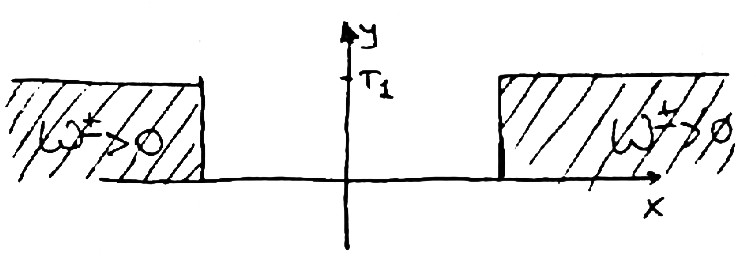
\includegraphics[scale=0.5]{14_2_new}
\end{center}
Но $\omega_{\varepsilon}^{\pm}(t,x)$ удовлетворяет уровнению теплопроводности $\Rightarrow$ на $\Gamma_{T_1}$ достигаются максимум и минимум 
$\omega_{\varepsilon}^{\pm}(t,x) \Rightarrow$ он строго $>0 \Rightarrow \omega_{\varepsilon}^{\pm}(t,x)>0$ всюду в полосе $(0,T_1)$.
Итак, $\mp v(t,x) \leq \varepsilon u_{2T_1}(t,x) \Rightarrow \abs*{v} \leq \varepsilon u_{2T_1}(t,x) \Forall \varepsilon > 0 \Rightarrow v\equiv 0$ в $\overline{\Pi_{T_1}}$
 
\end{proof}
\end{lemma}

\begin{theorem}
Задача Коши $\mathrm{L}u = f(x,t), \eval{u}_{t = 0} = u_0(x)$ в {\bf классе Тихонова} не может иметь более одного решения в полосе $\Pi_T$.

\begin{proof}
Пусть существует два решения: $u_1$ и $u_2$. Возьмем $v(t,x) = u_2 - u_1$. Функция $v$ удовлетворяет полностью однородной ЗК и лежит в {\bf классе Тихонова} 
$\Rightarrow$ в полосе $\Pi_{T_1}$, где $T_1$ определенно из предыдущей леммы, будет $v\equiv 0$.\\
Если $T \leq T_1$, то все доказано. В противном случае вводим:\\
$w(t,x) = v(t+T_1,x)$. Она удовлеворяет:
  \begin{equation}
  \begin{cases}
  w_t - a^2\Delta_xw=0,\\
  \eval{w}_{t=0} = 0, & T_1 \leq t < T, \, x \in \R^n.
  \end{cases}
  \end{equation}
$\Rightarrow$ в полосе $(0,T_1)$ получим $w \equiv 0$.\\
($T_1$ определяется $\dfrac{1}{8a^2\alpha} \Rightarrow$ одно и то же)\\
Так за конечное число шагов $N = \lceil{\frac{T}{T_1}} \rceil$ мы покроем всю $\Pi_T$.
\end{proof} 
\end{theorem}


\end{itemize}
